
\documentclass[12pt, letterpaper, twoside]{article}
\usepackage{graphicx}
\usepackage[utf8]{inputenc}
\usepackage{enumerate} % enumerados
\usepackage{multirow} % para las tablas
\usepackage{float} % para usar [H]
 
\title{Organizaci\'on y Arquitectura de computadoras Práctica 1}
\author{Arteaga Hernández Alejandro Iabin 313033414}
\date{18 de febrero de 2017}
 
\begin{document}
 
\maketitle

Nombre del alumno: Arteaga Hernández Alejandro  
hola
Datos de la computadora:
\begin{itemize}
    \item Fabricante y modelo de la computadora:
     
          DELL Optiplex-980
    \item Fabricante, modelo, frecuencia, número de núcleos, y arquitectura del procesador:
    
    Intel, Intel Core i5-660,3,33Ghz whitout overclocking, 4 cores, 64 bits.
    \item Capacidad de memoria RAM y de chachés de los procesadores:
    
    8192 Mb memoria RAM, 4 mb memoria caché del procesador.
    \item Capacidad, tipo y velocidad del disco duro:\\
    Seagate 975.2 GB  7200 Rpm Sata 
    
    \item Distribución de linux y versión del kernel:
    
    Ubuntu 16.10
\end{itemize}



\begin{table}[H]
\begin{center}
\begin{tabular}{|l|l|}
\hline
Nombre de la prueba & Resultado \\
\hline \hline
GZIP Compression & 15.25 Seconds \\ \hline
DCRAW & 75.12 Seconds \\ \hline
FLAC Audio Encoding & 8.85 Seconds \\ \hline
GnuPG & 16.30 Seconds\\  \hline
REDIS & 1516383.52 Requests Per Second \\ \hline
Timed MAFFT Alignment & 17.77 Seconds \\ \hline
Timed MrBayes Analysis & 44.41 Seconds \\ \hline
Timed M Player Compilation & 124.42 Seconds \\ \hline
Timed PHP Compilation & 68.34 Seconds\\ \hline
\end{tabular}
\caption{Resultado de las pruebas}
\label{tabla:sencilla}
\end{center}
\end{table}
 1.-Identifica que pruebas miden el tiempo de respuesta y cuales miden el rendimiento\\
 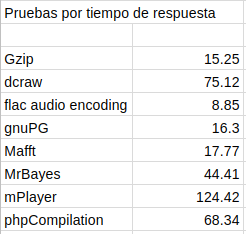
\includegraphics[scale=0.6]{respuesta.png}\\\\
 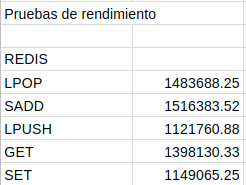
\includegraphics[scale=0.6]{rendimiento.png}\\
 2.-Usando las medias adecuadas calcula\\
 \begin{itemize}
    \item La media de tiempo de respuesta es :\\
    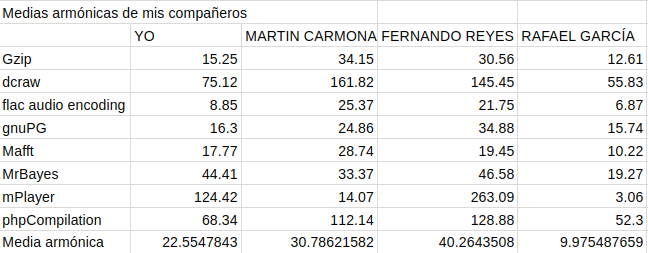
\includegraphics[scale=0.6]{media.png}\\
    \item la media de rendimiento es:\\\\
    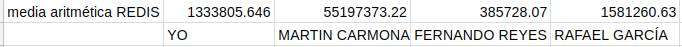
\includegraphics[scale=0.6]{rendimientoe.png}
\end{itemize}
 3.-Calcular los tiempos normalizados\\
 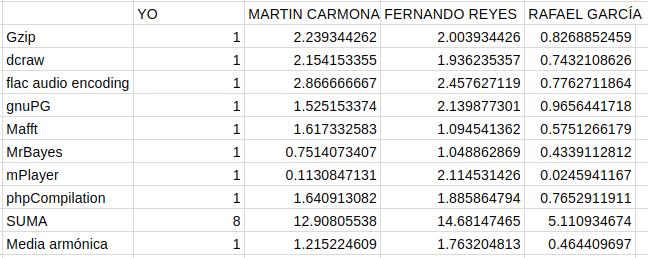
\includegraphics[scale=0.6]{NORMAL.png}\\\\
 4.-Casos de uso:\\ Aunque algunas pruebas me temo yo, están mal debido a que, se tarda extremadamente poco en algunos casos, no las tomaré en cuenta para esta parte, por ejemplo, si yo fuera un programador WEB, la computadora de RAFAEL sería la ideal, porque en la prueba del compilador de PHP fué la mas rápida, además de que para el procesamiento de imágenes etc, vendría muy bien, sin embargo, si quisiese poner un servidor web en mi casa, la computadora de MARTÍN sería la ideal, porque maneja muy rápido las peticiones SQL, además de que no necesita potencia de más, con esa computadora es más que suficiente, es la más accesible de todas y es sufiente. 
 Si quisiese una computadora para solamente escribir reportes en algún programa de ofimática, mi computadora sería ideal,ya que con poca o ninguna frecuencia, tendría que compilar algo y no es tan cara como la Rafael y cumple con el objetivo.\\\\
 
 \textbf{Preguntas}\\
 1.La computadora de RAFAEL tiene el mejor tiempo de ejecición(lower is better)
 \\
 “El tiempo de ejecución de la computadora de MARTÍN es 2.47 veces que el de la
computadora de RAFAEL”.(Quité la compilación de Mplayer, porque me pareció poco confiable que en la computadora de martín solo tardara 6 segs)
\\\\2.-La computadora de MARTÍN tiene mejor desempeño con 55197373.22 respuestas por segundo(Aunque aquí creo que volvieron a fallar las pruebas, porque me parece excesivo pero bueno :P)
\\ “El rendimiento de la computadora Martín es 143.099187 veces que la computadora de Reyes”.
\\(Sigo pensando que la prueba dió malos resultados)\\\\
\\3- De acuerdo a la computadora de referencia, ¿cual computadora tiene mejor desempeño y
cual computadora tiene el peor desempeño?\\
La que tiene mejor desempeño es la computadora de Rafael con 2.1532711455 del rendimiento de mi computadora
La que tiene peor desempeño es la computadora de Martín es 0.82289314465  del rendimiento de mi computadora\\\\
4.-La computadora de Rafael, es mejor en todos los casos de uso :v, pero en el ejercicio 4 detallé mas a fondo donde funcionaría mejor cada máquina 
\\\\
5.-EL atributo mas importante es el procesador, pero como siempre, es muy dependiente, depende de la capacidad de RAM o de su velocidad, si es una laptop o no etc. El que menos importancia tiene son los periféricos y el Disco duro, con una buena cantidad de RAM el disco duro su importancia se disminuye mucho en un procesamiento.
\end{document}

